\documentclass[12pt,a4paper]{article}
\usepackage[utf8]{inputenc}
\usepackage[T1]{fontenc}
\usepackage{amsmath,amssymb,amsfonts}
\usepackage{geometry}
\usepackage{listings}
\usepackage{xcolor}
\usepackage{hyperref}
\usepackage{booktabs}
\usepackage{array}
\usepackage{tikz}
\usetikzlibrary{arrows.meta,shapes,positioning,calc}

\geometry{margin=2.5cm}
\lstset{
  basicstyle=\ttfamily\footnotesize,
  keywordstyle=\color{blue!80}\bfseries,
  commentstyle=\color{gray}\itshape,
  stringstyle=\color{red!70},
  breaklines=true,
  frame=single,
  backgroundcolor=\color{gray!5},
  numbers=left,
  numberstyle=\tiny\color{gray},
  captionpos=b
}

\title{\textbf{Report 2: Total Energy Control System (TECS)}\\[0.4em]
\large \textbf{Part~I:} Complete Original System --- Every Function\\
\textbf{Part~II:} Every Soaring-Mode Modification and Its Physical Impact\\[0.5em]
\normalsize PX4 Autosoaring Implementation --- Defence Technical Report}
\author{Radhouene --- Fixed-Wing Autosoaring Project}
\date{April 2026}

\begin{document}
\maketitle
\tableofcontents
\newpage

%=============================================================================
\section*{List of Symbols}
\addcontentsline{toc}{section}{List of Symbols}
%=============================================================================

Throughout this report, the following notation is used consistently.
A hat $\hat{(\cdot)}$ denotes a Kalman-filter estimate.
A superscript $(\cdot)^-$ denotes a \emph{prior} (predicted before measurement update).
A superscript $(\cdot)^*$ denotes a \emph{setpoint} (commanded value).
A dot $\dot{(\cdot)}$ denotes the time derivative.

\subsection*{State Variables}
\begin{center}\begin{tabular}{lll}\toprule
Symbol & Meaning & Unit \\\midrule
$V$ & True airspeed (TAS) & m/s \\
$\dot{V}$ & TAS time derivative & m/s$^2$ \\
$V_{\text{EAS}}$ & Equivalent airspeed (EAS); corrected for air density & m/s \\
$\dot{V}_{\text{EAS}}$ & EAS time derivative & m/s$^2$ \\
$\hat{V}_{\text{EAS}}$ & Kalman-filter estimate of EAS & m/s \\
$\hat{\dot{V}}_{\text{EAS}}$ & Kalman-filter estimate of EAS rate & m/s$^2$ \\
$\hat{\mathbf{x}}$ & Filter state vector $(\hat{V}_{\text{EAS}},\,\hat{\dot{V}}_{\text{EAS}})^\top$ & --- \\
$\hat{\mathbf{x}}^-$ & Prior (predicted) state vector before measurement update & --- \\
$h$ & Altitude above mean sea level (AMSL) & m \\
$\dot{h}$ & Altitude rate (positive = climbing) & m/s \\
$\theta$ & Pitch angle & rad \\
$\phi$ & Bank (roll) angle & rad \\
\bottomrule\end{tabular}\end{center}

\subsection*{Setpoints and Reference Signals}
\begin{center}\begin{tabular}{lll}\toprule
Symbol & Meaning & Unit \\\midrule
$V^*$, $V^*_{\text{TAS}}$ & TAS setpoint (commanded) & m/s \\
$V^*_{\text{EAS}}$ & EAS setpoint & m/s \\
$\dot{V}^*$ & Demanded airspeed rate & m/s$^2$ \\
$\dot{V}^*_{\max}$, $\dot{V}^*_{\min}$ & Upper/lower bounds on demanded airspeed rate & m/s$^2$ \\
$h^*$ & Altitude setpoint from navigator & m \\
$h_{\text{ref}}$ & Jerk-limited altitude reference from trajectory model & m \\
$\dot{h}_{\text{ref}}$ & Altitude rate of the trajectory reference model & m/s \\
$\dot{h}^*$ & Demanded altitude rate & m/s \\
$\theta^*$ & Pitch setpoint & rad \\
$\delta_t$ & Throttle setpoint (0 = idle, 1 = full) & --- \\
$\delta_{t,\text{pred}}$ & Bilinear feed-forward throttle prediction & --- \\
$\tilde{\dot{B}}$ & SEB rate control error $= \dot{B}_{\text{sp}} - \dot{B}_{\text{est}}$ & m$^2$/s$^3$ \\
$\tilde{\dot{E}}$ & STE rate control error $= \dot{E}^*_{\text{STE}} - \hat{\dot{E}}$ & m$^2$/s$^3$ \\
\bottomrule\end{tabular}\end{center}

\subsection*{Energy Quantities}
\begin{center}\begin{tabular}{lll}\toprule
Symbol & Meaning & Unit \\\midrule
$E_k = V^2/(2g)$ & Specific kinetic energy (per unit weight) & m \\
$E_p = h$ & Specific potential energy & m \\
$E = E_k + E_p$ & Total specific energy & m \\
$\dot{E}_k = V\dot{V}/g$ & Specific kinetic energy rate & m$^2$/s$^3$ \\
$\dot{E}_p = \dot{h}$ & Specific potential energy rate (altitude rate) & m$^2$/s$^3$ \\
$\dot{E} = \dot{E}_k + \dot{E}_p$ & Total specific energy rate & m$^2$/s$^3$ \\
$\dot{E}_{\max}$ & Maximum reachable STE rate (max climb $\times g$) & m$^2$/s$^3$ \\
$\dot{E}_{\min}$ & Minimum reachable STE rate (max sink $\times g$, negative) & m$^2$/s$^3$ \\
$\hat{\dot{E}}$ & Low-pass filtered STE rate estimate & m$^2$/s$^3$ \\
$\dot{B}$ & Specific energy balance (SEB) rate $= w_{\text{spe}}\dot{E}_p - w_{\text{ske}}\dot{E}_k$ & m$^2$/s$^3$ \\
$\dot{B}_{\text{sp}}$ & SEB rate setpoint (from weighted setpoint quantities) & m$^2$/s$^3$ \\
$\dot{B}_{\text{est}}$ & SEB rate estimate (from weighted measured quantities) & m$^2$/s$^3$ \\
$\dot{E}_{p/k,\text{sp}}$ & Potential/kinetic SER setpoint component & m$^2$/s$^3$ \\
$\dot{E}_{p/k,\text{est}}$ & Potential/kinetic SER estimated component & m$^2$/s$^3$ \\
$\dot{E}^*_{\text{STE}}$ & STE rate setpoint (with load-factor correction) & m$^2$/s$^3$ \\
\bottomrule\end{tabular}\end{center}

\subsection*{Weighting and Control Gains}
\begin{center}\begin{tabular}{lll}\toprule
Symbol & Meaning & Unit \\\midrule
$w_{\text{spe}}$ & Altitude (potential energy) weight on pitch loop, $\in[0,2]$ & --- \\
$w_{\text{ske}}$ & Airspeed (kinetic energy) weight on pitch loop, $\in[0,2]$ & --- \\
$w_p$ & Speed priority parameter (\texttt{FW\_T\_SPDWEIGHT}); $w_{\text{ske}}=w_p$, $w_{\text{spe}}=2-w_p$ & --- \\
$k_V = 1/\tau_V$ & Airspeed proportional gain (\texttt{airspeed\_error\_gain}) & s$^{-1}$ \\
$k_h = 1/\tau_h$ & Altitude proportional gain (\texttt{altitude\_error\_gain}) & s$^{-1}$ \\
$k_{\text{ff}}$ & Altitude feedforward gain (\texttt{altitude\_setpoint\_gain\_ff}) & --- \\
$K_{i,\theta}$ & Pitch integrator gain (\texttt{integrator\_gain\_pitch}) & --- \\
$K_{i,t}$ & Throttle integrator gain (\texttt{integrator\_gain\_throttle}) & --- \\
$K_d$ (pitch) & Pitch damping gain (\texttt{pitch\_damping\_gain}) & --- \\
$K_{\text{ff}}$ (pitch) & SEB rate feedforward gain (\texttt{seb\_rate\_ff}) & --- \\
$K_{\text{damp}}$ & Throttle damping gain (\texttt{throttle\_damping\_gain}) & --- \\
$K_{\text{STE}}$ & STE rate error to throttle scaler $= 1/(\dot{E}_{\max}-\dot{E}_{\min})$ & s$^3$/m$^2$ \\
$K_{\delta,+}$ & Throttle slope above trim $= (\delta_{t,\max}-\delta_{t,\text{trim}})/\dot{E}_{\max}$ & --- \\
$K_{\delta,-}$ & Throttle slope below trim $= (\delta_{t,\text{trim}}-\delta_{t,\min})/|\dot{E}_{\min}|$ & --- \\
$K_{\text{lf}}$ & Load-factor STE rate correction gain (\texttt{load\_factor\_correction}) & m$^2$/s$^3$ \\
\bottomrule\end{tabular}\end{center}

\subsection*{Integrators}
\begin{center}\begin{tabular}{lll}\toprule
Symbol & Meaning & Unit \\\midrule
$I_\theta$ & Pitch integrator state (\texttt{\_pitch\_integ\_state}) & rad \\
$I_t$ & Throttle integrator state (\texttt{\_throttle\_integ\_state}) & --- \\
\bottomrule\end{tabular}\end{center}

\subsection*{Kalman Filter Notation (TECSAirspeedFilter)}
\begin{center}\begin{tabular}{lll}\toprule
Symbol & Meaning & Unit \\\midrule
$\sigma_V$ & Airspeed measurement noise std.\ deviation & m/s \\
$\sigma_{\dot{V}}$ & Airspeed \emph{rate} measurement noise std.\ deviation & m/s$^2$ \\
$\sigma_q$ & Airspeed rate process noise std.\ deviation (model uncertainty) & m/s$^2$ \\
$K_c$ & Continuous Kalman gain matrix ($2\!\times\!2$) from CARE solution & --- \\
$K_d = \Delta t\cdot K_c$ & Discrete Kalman gain matrix & --- \\
$\boldsymbol{\nu}$ & Innovation (measurement residual) vector & --- \\
$D, C, R_-$ & Intermediate scalar quantities in CARE solution (defined locally) & --- \\
\bottomrule\end{tabular}\end{center}

\subsection*{Physical and Aircraft Parameters}
\begin{center}\begin{tabular}{lll}\toprule
Symbol & Meaning & Unit \\\midrule
$g = 9.81$ & Gravitational acceleration & m/s$^2$ \\
$m$ & Aircraft mass & kg \\
$\rho$ & Local air density at current altitude & kg/m$^3$ \\
$\rho_0 = 1.225$ & ISA sea-level air density & kg/m$^3$ \\
$k = k_{\text{EAS2TAS}} = \sqrt{\rho_0/\rho}$ & EAS-to-TAS conversion factor ($\geq 1$) & --- \\
$n_z = 1/\cos\phi$ & Normal load factor in banked flight & --- \\
$V_{\text{trim}}$ & Trim (cruise) EAS; aircraft flies level at idle trim & m/s \\
$V_{\text{EAS,min}}$, $V_{\text{EAS,max}}$ & Minimum and maximum EAS flight envelope limits & m/s \\
$V_{\text{TAS,min}}$, $V_{\text{TAS,max}}$ & Minimum and maximum TAS limits & m/s \\
$\delta_{t,\text{trim}}$ & Throttle at trim speed, level flight & --- \\
$\delta_{t,\min}$, $\delta_{t,\max}$ & Throttle lower/upper bounds & --- \\
$\theta_{\min}$, $\theta_{\max}$ & Pitch angle lower/upper bounds & rad \\
$a_{z,\text{lim}}$ & Vertical acceleration limit (\texttt{FW\_T\_VERT\_ACC}) & m/s$^2$ \\
$\dot{h}_{\text{climb,max}}$ & Maximum achievable climb rate (\texttt{FW\_T\_CLMB\_MAX}) & m/s \\
$\dot{h}_{\text{sink,min}}$ & Minimum sink rate at best glide (positive) (\texttt{FW\_T\_SINK\_MIN}) & m/s \\
$\dot{h}_{\text{sink,max}}$ & Maximum allowable sink rate (\texttt{FW\_T\_SINK\_MAX}) & m/s \\
$\dot{h}_{\text{climb,target}}$ & Target (desired) climb rate, $\leq\dot{h}_{\text{climb,max}}$ & m/s \\
$\dot{h}_{\text{sink,target}}$ & Target sink rate, $\leq\dot{h}_{\text{sink,max}}$ & m/s \\
\bottomrule\end{tabular}\end{center}

\subsection*{Time Constants and Intervals}
\begin{center}\begin{tabular}{lll}\toprule
Symbol & Meaning & Unit \\\midrule
$\Delta t$ & Control cycle interval (clamped to [1\,ms, 1\,s]) & s \\
$\tau_V$ & Airspeed error time constant (\texttt{FW\_T\_TAS\_ERROR\_TC}, default 10\,s) & s \\
$\tau_h$ & Altitude error time constant (\texttt{FW\_T\_H\_ERROR\_TC}, default 5\,s) & s \\
$\tau_{\text{STE}}$ & STE rate LP filter time constant (\texttt{STE\_RATE\_TC}, default 0.1\,s) & s \\
$\tau$ & Throttle integrator decay time constant (\texttt{FW\_GLIDE\_I\_DECAY}) & s \\
$T_{\text{ramp}}$ & Fast-descend ramp-up time ($\texttt{FAST\_DESCEND\_RAMP\_UP\_TIME} = 2$\,s) & s \\
DT\_MIN & Minimum cycle time guard = 1\,ms & s \\
DT\_MAX & Maximum cycle time guard = 1\,s (triggers full reset) & s \\
\bottomrule\end{tabular}\end{center}

\subsection*{Underspeed Detection}
\begin{center}\begin{tabular}{lll}\toprule
Symbol & Meaning & Unit \\\midrule
$r_u \in [0,1]$ & Underspeed ratio: 0 = no underspeed, 1 = fully undersped & --- \\
$p_{\text{err}} = 0.15$ & Airspeed error percentage for underspeed boundary computation & --- \\
$\varepsilon_V$ & Airspeed error bound $= p_{\text{err}}\cdot V_{\text{trim}}$ & m/s \\
$V_{\text{fully}}$ & TAS at which aircraft is fully undersped $= \max(V_{\text{TAS,min}}-2\varepsilon_V,0)$ & m/s \\
$V_{\text{start}}$ & TAS at which underspeed begins $= \max(V_{\text{TAS,min}}-\varepsilon_V,V_{\text{fully}})$ & m/s \\
\bottomrule\end{tabular}\end{center}

\subsection*{Fast-Descend Mode}
\begin{center}\begin{tabular}{lll}\toprule
Symbol & Meaning & Unit \\\midrule
$\alpha_{\text{fd}} \in [0,1]$ & Fast-descend blend factor: 0 = normal, 1 = full fast-descend & --- \\
$h_{\text{err,fd}}$ & Altitude error threshold activating fast-descend (\texttt{FW\_T\_FAST\_ALT\_ERR}) & m \\
\bottomrule\end{tabular}\end{center}

\subsection*{Trajectory Generators (TECSAltitudeReferenceModel)}
\begin{center}\begin{tabular}{lll}\toprule
Symbol & Meaning & Unit \\\midrule
$j_{\max}$ & Maximum jerk of trajectory generator (\texttt{jerk\_max}) & m/s$^3$ \\
$a_{\max}$ & Maximum vertical acceleration (\texttt{vert\_accel\_limit}) & m/s$^2$ \\
$\delta h$ & Altitude error to setpoint $= h^*_{\text{nav}} - h_{\text{traj,current}}$ & m \\
$h_{\text{vel}}$ & Altitude integrated from velocity generator & m \\
$h_{\text{traj,current}}$ & Current position of altitude-control trajectory generator & m \\
\bottomrule\end{tabular}\end{center}

\subsection*{Glide Polar (Part~II)}
\begin{center}\begin{tabular}{lll}\toprule
Symbol & Meaning & Unit \\\midrule
$a$ & Induced drag coefficient of glide polar; $w_s = aV^2 + b$ & s$^2$/m$^2$ (or 1/(m$\cdot$s)) \\
$b$ & Profile drag coefficient of glide polar & m/s \\
$w_s(V)$ & Sink rate at airspeed $V$; $w_s = aV^2 + b$ (positive downward) & m/s \\
$V^*_{\text{EAS,polar}}$ & Best-glide EAS from polar minimum $= \sqrt{b/a}$ & m/s \\
$(L/D)_{\max}$ & Maximum lift-to-drag ratio $= 1/(2\sqrt{ab})$ & --- \\
$V_{\text{TAS,stall,banked}}$ & Banked stall TAS $= V_{\text{TAS,min}}\sqrt{n_z}$ & m/s \\
\bottomrule\end{tabular}\end{center}

\subsection*{Mathematical Operators}

\begin{center}
\begin{tabular}{p{2.5cm} p{8cm} p{5cm}}
\toprule
Operator & Meaning & Notes \\
\midrule
$\text{clamp}(x,\,a,\,b)$ & Saturate: $\max(a,\min(b,x))$ & Also written \texttt{constrain} in PX4 \\
$\text{lerp}(a,b,t)$ & Linear interpolation: $(1-t)a + tb$ & $t\in[0,1]$; also \texttt{lerp()} in PX4 \\
$\text{sign}(x)$ & Signum: $+1$ if $x>0$, $-1$ if $x<0$, $0$ if $x=0$ & \\
$\varepsilon$ & Positive float machine epsilon / guard value & Used in division denominators \\
$\max(a,b)$, $\min(a,b)$ & Standard maximum / minimum & \\
$|x|$, $\text{fabsf}(x)$ & Absolute value & \\
\bottomrule
\end{tabular}
\end{center}

\newpage
% ============================================================
%  PART I  — ORIGINAL SYSTEM (every function)
% ============================================================
\part{Original TECS System}

%=============================================================================
\section{Physical Background}
%=============================================================================

TECS (Total Energy Control System), originally proposed by A.~A.~Lambregts
(1983), controls a fixed-wing aircraft's airspeed and altitude simultaneously
by separating them into two energy channels.

\subsection{Specific Energy Definitions}

Let $m$ = aircraft mass, $g = 9.81\,\text{m/s}^2$, $V$ = true airspeed,
$h$ = altitude. Specific energies (per unit weight $mg$):

\begin{align}
  E_k &= \frac{V^2}{2g} \quad [\text{m, kinetic}] \\
  E_p &= h \quad [\text{m, potential}] \\
  E   &= E_k + E_p \quad [\text{m, total}]
\end{align}

Specific energy rates $[\text{m}^2/\text{s}^3]$:
\begin{align}
  \dot{E}_k &= \frac{V\dot{V}}{g}, \qquad
  \dot{E}_p = \dot{h}, \qquad
  \dot{E}   = \dot{E}_k + \dot{E}_p
\end{align}

Specific energy balance rate (SEB):
\begin{equation}
  \dot{B} = w_{\text{spe}}\,\dot{E}_p - w_{\text{ske}}\,\dot{E}_k
  \label{eq:seb}
\end{equation}

with $w_{\text{spe}} + w_{\text{ske}} = 2$.

\subsection{Two-Channel Decoupling}

\begin{center}
\begin{tabular}{lll}
\toprule
Energy quantity & Controlled by & Physical action \\
\midrule
$\dot{E} = \dot{E}_k + \dot{E}_p$ & \textbf{Throttle} & Add/remove total energy \\
$\dot{B} = w_{\text{spe}}\dot{E}_p - w_{\text{ske}}\dot{E}_k$ & \textbf{Pitch} & Redistribute energy \\
\bottomrule
\end{tabular}
\end{center}

%=============================================================================
\section{Class Architecture}
%=============================================================================

Four cooperating C++ classes:

\begin{center}
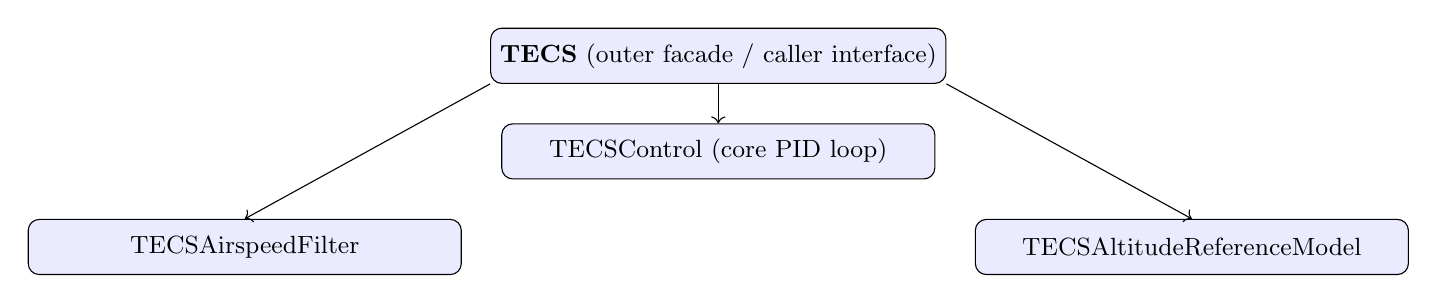
\begin{tikzpicture}[node distance=1.1cm,
  cls/.style={draw,rounded corners,fill=blue!8,minimum width=5.5cm,
              minimum height=0.7cm,align=center,font=\small}]
  \node[cls] (tecs) {\textbf{TECS} (outer facade / caller interface)};
  \node[cls,below=0.5cm of tecs] (ctrl) {TECSControl (core PID loop)};
  \node[cls,below left=0.5cm and 0.5cm of ctrl] (filt) {TECSAirspeedFilter};
  \node[cls,below right=0.5cm and 0.5cm of ctrl] (ref) {TECSAltitudeReferenceModel};
  \draw[->] (tecs) -- (ctrl);
  \draw[->] (tecs.south west) -- (filt.north);
  \draw[->] (tecs.south east) -- (ref.north);
\end{tikzpicture}
\end{center}

The outer \texttt{TECS} facade owns one instance of each submodule and is
the only class called by \texttt{FixedwingPositionControl}.

%=============================================================================
\section{Class 1: TECSAirspeedFilter}
%=============================================================================

\subsection{initialize()}

\begin{lstlisting}[language=C++]
void TECSAirspeedFilter::initialize(
    const float equivalent_airspeed,
    const float equivalent_airspeed_trim,
    const bool  airspeed_sensor_available)
\end{lstlisting}

Called when TECS is first started or after a long update gap
($\Delta t > \text{DT\_MAX} = 1\,\text{s}$).

\begin{itemize}
  \item If sensor available AND EAS is finite:
        $\hat{V}_{\text{EAS}} \leftarrow$ \texttt{equivalent\_airspeed}.
  \item Otherwise: $\hat{V}_{\text{EAS}} \leftarrow$ \texttt{equivalent\_airspeed\_trim}
        (trim fallback prevents NaN initialisation).
  \item Always: $\hat{\dot{V}}_{\text{EAS}} \leftarrow 0$.
\end{itemize}

\textbf{Effect:} On the first update cycle after reset, the filter starts
from a known-good state rather than an uninitialised value.

\subsection{update()}

Called every TECS cycle with:
\begin{itemize}
  \item \texttt{dt} = elapsed time [s].
  \item \texttt{input.equivalent\_airspeed} = raw EAS measurement.
  \item \texttt{input.equivalent\_airspeed\_rate} = raw EAS rate
        ($\dot{V}_{\text{EAS}}$ from forward-filtered accelerometer).
  \item \texttt{param} = Kalman noise parameters.
  \item \texttt{airspeed\_sensor\_available} = validity flag.
\end{itemize}

\paragraph{Input guard:} If \texttt{dt} is not a valid timestamp
(\texttt{TIMESTAMP\_VALID(dt)} fails), the function returns immediately
with a warning and the state is unchanged.

\paragraph{Sensor fallback:}
\begin{itemize}
  \item If sensor unavailable or EAS not finite:
        measurement $\leftarrow V_{\text{trim}}$,
        rate measurement $\leftarrow 0$.
\end{itemize}

\paragraph{Prediction step (constant-rate model):}
\begin{equation}
  \hat{\mathbf{x}}^- =
  \begin{pmatrix} \hat{V} + \Delta t\,\hat{\dot{V}} \\ \hat{\dot{V}} \end{pmatrix}
\end{equation}

\paragraph{Kalman gain (solved from continuous Riccati equation):}

Define:
\begin{align}
  \sigma_V^{-1} &= 1/\sigma_V \quad\text{(speed noise inverse)} \\
  R_{-} &= \sigma_{\dot{V}}^{-2}\,\sigma_q \quad\text{(rate-noise-normalised process)} \\
  D     &= \sigma_V^{-1} + R_{-} \\
  C     &= \sqrt{\sigma_q\,(2\sigma_V^{-1} + R_{-})}
\end{align}

The $2\times 2$ discrete gain is $K_d = \Delta t \cdot K_c$:
\begin{equation}
  K_d = \Delta t \cdot
  \begin{pmatrix}
    \sigma_V^{-1} C / D & R_{-}/D \\
    \sigma_V^{-2}\sigma_q/D & R_{-}C/D
  \end{pmatrix}
\end{equation}

\paragraph{Innovation vector:}
\begin{equation}
  \boldsymbol{\nu} =
  \begin{pmatrix} V_{\text{meas}} - \hat{V}^- \\ \dot{V}_{\text{meas}} - \hat{\dot{V}}^- \end{pmatrix}
\end{equation}

\paragraph{Update step:}
\begin{equation}
  \hat{\mathbf{x}} = \hat{\mathbf{x}}^- + K_d\,\boldsymbol{\nu}
\end{equation}

\paragraph{Airspeed floor and rate correction:}
If the updated speed $\hat{V} < \varepsilon$ (negative due to noise):
\begin{itemize}
  \item Set $\hat{V} \leftarrow 0$.
  \item Back-calculate the innovation that \emph{would} produce $\hat{V} = 0$:
        \begin{equation}
          \nu_V^{\text{zero}} = \frac{-\hat{V}^-/\Delta t - K_d(0,1)\,\nu_{\dot{V}}}{K_d(0,0)}
        \end{equation}
  \item Recompute $\hat{\dot{V}}$ using this adjusted innovation (prevents
        physically inconsistent negative-speed states with non-zero acceleration).
\end{itemize}

\paragraph{State update:}
\begin{align}
  \texttt{\_airspeed\_state.speed}      &\leftarrow \hat{V} \\
  \texttt{\_airspeed\_state.speed\_rate} &\leftarrow \hat{\dot{V}}
\end{align}

\subsection{getState()}

Returns the private \texttt{\_airspeed\_state} struct
(speed $+$ speed\_rate) for use by the TECS facade when building the
\texttt{TECSControl::Input}:
\begin{equation}
  V_{\text{TAS}} = k \cdot \hat{V}_{\text{EAS}}, \qquad
  \dot{V}_{\text{TAS}} = k \cdot \hat{\dot{V}}_{\text{EAS}}
  \quad k = k_{\text{EAS2TAS}}
\end{equation}

%=============================================================================
\section{Class 2: TECSAltitudeReferenceModel}
%=============================================================================

\subsection{initialize()}

\begin{lstlisting}[language=C++]
void TECSAltitudeReferenceModel::initialize(
    const AltitudeReferenceState &state)
\end{lstlisting}

Called on TECS reset or during glide (see Part~II, M1).

\begin{itemize}
  \item NaN guard: if \texttt{state.alt} or \texttt{state.alt\_rate} is
        not finite, use 0.
  \item Calls \texttt{reset(jerk=0, vel=alt\_rate, pos=alt)} on both
        trajectory generators: \texttt{\_alt\_control\_traj\_generator}
        and \texttt{\_velocity\_control\_traj\_generator}.
\end{itemize}

After initialisation, both generators report:
$h_{\text{ref}} = h$, $\dot{h}_{\text{ref}} = \dot{h}$ (current state).

\subsection{update() --- The Two Trajectory Generators}

\begin{lstlisting}[language=C++]
void TECSAltitudeReferenceModel::update(
    const float dt,
    const AltitudeReferenceState &setpoint,
    float altitude, float height_rate,
    const Param &param)
\end{lstlisting}

\paragraph{Input guard:} Returns immediately if \texttt{dt} invalid.

\paragraph{Common jerk/accel/velocity limits pushed each cycle:}

\begin{center}
\begin{tabular}{ll}
\toprule
Generator & Limits set \\
\midrule
\texttt{\_velocity\_control\_traj\_generator} & MaxJerk, MaxAccelUp/Down, MaxVelUp/Down \\
\texttt{\_alt\_control\_traj\_generator} & MaxJerk, MaxAccel, MaxVel \\
\bottomrule
\end{tabular}
\end{center}

Note: the velocity generator uses inverted sign convention:
\texttt{MaxVelUp} $= \dot{h}_{\text{sink,max}}$,
\texttt{MaxVelDown} $= \dot{h}_{\text{climb,max}}$
(because the velocity generator uses NED z-axis convention).

\paragraph{Two operating modes, selected by \texttt{setpoint.alt\_rate}:}

\subparagraph{Mode A: Height-rate control (alt\_rate is finite)}

\begin{enumerate}
  \item Velocity generator updated:
        $\texttt{\_velocity\_control\_traj\_generator.update}(\Delta t, \dot{h}^*)$
  \item This integrates the jerk-limited velocity profile to produce a
        jerk-limited altitude trajectory:
        $h_{\text{vel}} = \int \dot{h}_{\text{jerk-limited}}\,dt$
  \item If $h_{\text{vel}}$ is finite: altitude setpoint locked
        (\texttt{control\_altitude = true}).
  \item Otherwise: altitude-control generator stays at current altitude;
        \texttt{\_height\_rate\_setpoint\_direct} is set to the
        velocity generator's current velocity output
        (passed directly to TECSControl bypassing the altitude P loop).
\end{enumerate}

\subparagraph{Mode B: Altitude control (alt\_rate is NaN)}

\begin{enumerate}
  \item Velocity generator is reset (does not integrate):
        $\texttt{reset}(0, \dot{h}_{\text{meas}}, h^*_{\text{nav}})$.
  \item Altitude-control generator receives $h^*$ from navigator.
  \item Jerk-limited height rate target:
        \begin{equation}
          \dot{h}_{\text{target}} = \text{sign}(\delta h) \cdot
            \texttt{computeMaxSpeedFromDistance}(j_{\max}, a_{\max}, |\delta h|, 0)
        \end{equation}
        where $\delta h = h^*_{\text{nav}} - h_{\text{traj,current}}$.
        This function computes the maximum speed reachable from the
        current distance with jerk and acceleration limits
        (minimum-time bang-bang profile).
  \item Height rate clamped:
        $\dot{h}_{\text{target}} \leftarrow \text{clamp}(\dot{h}_{\text{target}},
        -\dot{h}_{\text{sink,target}}, \dot{h}_{\text{climb,target}})$
  \item Trajectory generator advanced: \texttt{updateDurations} + \texttt{updateTraj}.
  \item \texttt{\_height\_rate\_setpoint\_direct = NAN} (altitude loop
        will run in TECSControl via altitude P controller).
\end{enumerate}

\subsection{getAltitudeReference()}

Returns:
\begin{equation}
  \bigl(h_{\text{ref}},\,\dot{h}_{\text{ref}}\bigr)
  = \bigl(\texttt{\_alt\_control\_traj\_generator.getCurrentPosition()},\;
           \texttt{getCurrentVelocity()}\bigr)
\end{equation}

\subsection{getHeightRateSetpointDirect()}

Returns \texttt{\_height\_rate\_setpoint\_direct}:
\begin{itemize}
  \item NaN in altitude-control mode (TECSControl uses altitude P loop).
  \item Current velocity of the velocity generator in height-rate mode
        (TECSControl uses this directly, bypassing the altitude P loop).
\end{itemize}

%=============================================================================
\section{Class 3: TECSControl --- All Functions}
%=============================================================================

\subsection{resetIntegrals()}

\begin{lstlisting}[language=C++]
void TECSControl::resetIntegrals()
{
    _pitch_integ_state    = 0.0f;
    _throttle_integ_state = 0.0f;
}
\end{lstlisting}

Zeros both integrators. Called by:
\begin{itemize}
  \item \texttt{TECSControl::initialize()} (cold start / after reset).
  \item Externally via \texttt{TECS::initialize()}.
\end{itemize}

\subsection{initialize()}

\begin{lstlisting}[language=C++]
void TECSControl::initialize(const Setpoint &setpoint,
    const Input &input, Param &param, const Flag &flag)
\end{lstlisting}

Called only on TECS reset (first call or after DT\_MAX exceeded).
Does \textbf{not} run integrators. Its purpose is to compute valid
\emph{initial} setpoints so that the \emph{first} normal update cycle
does not start from undefined values.

\begin{enumerate}
  \item \texttt{resetIntegrals()}: zero both integrators.
  \item Run \texttt{\_calcAirspeedControlOutput()} to get $\dot{V}^*$.
  \item Run \texttt{\_calcAltitudeControlOutput()} to get $\dot{h}^*$.
  \item Compute \texttt{SpecificEnergyRates} from these.
  \item Run \texttt{\_detectUnderspeed()} (so $r_u$ is valid).
  \item Compute energy weights and SEB rate (no integrator update).
  \item Compute initial pitch setpoint $\theta^*$ using
        \texttt{\_calcPitchControlOutput()} (output only, no integrator).
  \item Reset the STE rate LP filter:
        $\texttt{\_ste\_rate\_estimate\_filter.reset}(\dot{E}_{p,\text{est}}
        + \dot{E}_{k,\text{est}})$.
  \item Compute initial throttle using
        \texttt{\_calcThrottleControlSteRate()} and
        \texttt{\_calcThrottleControlOutput()}.
  \item Populate debug output fields.
\end{enumerate}

\textbf{Key distinction from update():} no integrator update is performed.
The purpose is \emph{state initialisation}, not control.

\subsection{update()}

\begin{lstlisting}[language=C++]
void TECSControl::update(const float dt,
    const Setpoint &setpoint, const Input &input,
    Param &param, const Flag &flag)
\end{lstlisting}

\paragraph{Input guard:} If \texttt{dt} invalid, return immediately.

\paragraph{Build \texttt{AltitudePitchControl control\_setpoint}:}
\begin{enumerate}
  \item $\dot{V}^* \leftarrow$ \texttt{\_calcAirspeedControlOutput()}.
  \item Height-rate source selection:
        \begin{itemize}
          \item If \texttt{setpoint.altitude\_rate\_setpoint\\\_direct} is finite:
                $\dot{h}^* \leftarrow \texttt{altitude\_rate\_setpoint\_direct}$
                (direct height-rate control: altitude P loop bypassed).
          \item Else: $\dot{h}^* \leftarrow$ \texttt{\_calcAltitudeControlOutput()}
                (altitude P loop with FOH feedforward).
        \end{itemize}
\end{enumerate}

\paragraph{Run the 6 stages:}
\begin{enumerate}
  \item \texttt{\_calcSpecificEnergyRates()} --- build the four SER components.
  \item \texttt{\_detectUnderspeed()} --- update $r_u$.
  \item \texttt{\_calcPitchControl()} --- run pitch PID.
  \item \texttt{\_calcThrottleControl()} --- run throttle PID.
\end{enumerate}

\paragraph{Debug output fields:}

\begin{lstlisting}[language=C++]
_debug_output.altitude_rate_control           = control_setpoint.altitude_rate_setpoint;
_debug_output.true_airspeed_derivative_control = control_setpoint.tas_rate_setpoint;
_debug_output.pitch_integrator                = _pitch_integ_state;
_debug_output.throttle_integrator             = _throttle_integ_state;
\end{lstlisting}

%=============================================================================
\section{Internal Stage 0: \_calculateTotalEnergyRateLimit()}
%=============================================================================

\begin{lstlisting}[language=C++]
STERateLimit TECSControl::_calculateTotalEnergyRateLimit(
    const Param &param) const
\end{lstlisting}

Called at the beginning of Stage 1 (airspeed) and Stage 6 (throttle).

\begin{align}
  \dot{E}_{\max} &= \max(\dot{h}_{\text{climb,max}},\,\varepsilon) \cdot g \quad [\text{m}^2/\text{s}^3] \\
  \dot{E}_{\min} &= -\max(\dot{h}_{\text{sink,min}},\,\varepsilon) \cdot g \quad [\text{m}^2/\text{s}^3]
\end{align}

These define the physically reachable STE rate envelope.
$\dot{h}_{\text{climb,max}}$ comes from \texttt{FW\_T\_CLMB\_MAX} and
$\dot{h}_{\text{sink,min}}$ from \texttt{FW\_T\_SINK\_MIN}.

%=============================================================================
\section{Internal Stage 1: \_calcAirspeedControlOutput()}
%=============================================================================

\begin{lstlisting}[language=C++]
float TECSControl::_calcAirspeedControlOutput(
    const Setpoint &setpoint, const Input &input,
    const Param &param, const Flag &flag) const
\end{lstlisting}

\paragraph{No sensor path:} If \texttt{!flag.airspeed\_enabled}: return $0$.

\paragraph{Compute speed-rate limits from energy limits:}
\begin{align}
  \dot{V}^*_{\max} &= \frac{(0.5\,\alpha_{\text{fd}} + 0.5)\,\dot{E}_{\max}}{\max(V,\varepsilon)} \\
  \dot{V}^*_{\min} &= \frac{(0.5\,\alpha_{\text{fd}} + 0.5)\,\dot{E}_{\min}}{\max(V,\varepsilon)}
\end{align}

$\alpha_{\text{fd}} \in [0,1]$ is the fast-descend blend factor.
At $\alpha_{\text{fd}} = 0$ (normal flight), the factor is 0.5,
giving a 50\% margin relative to the physical limit.

\paragraph{Proportional speed error:}
\begin{equation}
  \dot{V}^* = \text{clamp}\!\left[(V^* - V)\,k_V,\;\dot{V}^*_{\min},\;\dot{V}^*_{\max}\right]
\end{equation}

$k_V = 1/\tau_V$ (\texttt{airspeed\_error\_gain}, default $\tau_V = 10\,\text{s}$).

%=============================================================================
\section{Internal Stage 2: \_calcAltitudeControlOutput()}
%=============================================================================

\begin{lstlisting}[language=C++]
float TECSControl::_calcAltitudeControlOutput(
    const Setpoint &setpoint, const Input &input,
    const Param &param) const
\end{lstlisting}

Proportional altitude outer-loop with feedforward:
\begin{equation}
  \dot{h}^* = k_h\,(h_{\text{ref}} - h) + k_{\text{ff}}\,\dot{h}_{\text{ref}}
\end{equation}

$k_h = 1/\tau_h$ (\texttt{altitude\_error\_gain}, default $\tau_h = 5\,\text{s}$),
$k_{\text{ff}}$ = \texttt{altitude\_setpoint\_gain\_ff}.

Clamped: $\dot{h}^* \leftarrow \text{clamp}(\dot{h}^*, -\dot{h}_{\text{sink,max}}, \dot{h}_{\text{climb,max}})$.

\textbf{Note:} This function is \emph{only} called when
\texttt{altitude\_rate\_setpoint\_direct} is NaN.
When finite, the reference model's height rate is used directly
(see \texttt{TECSControl::update()}, Stage 2).

%=============================================================================
\section{Internal Stage 3: \_calcSpecificEnergyRates()}
%=============================================================================

\begin{lstlisting}[language=C++]
SpecificEnergyRates TECSControl::_calcSpecificEnergyRates(
    const AltitudePitchControl &control_setpoint,
    const Input &input) const
\end{lstlisting}

Computes all four specific energy rate components:
\begin{align}
  \dot{E}_{p,\text{sp}}  &= \dot{h}^* \cdot g \quad [\text{m}^2/\text{s}^3] \\
  \dot{E}_{k,\text{sp}}  &= V^*_{\text{TAS}} \cdot \dot{V}^* \\
  \dot{E}_{p,\text{est}} &= \dot{h} \cdot g \\
  \dot{E}_{k,\text{est}} &= V_{\text{TAS}} \cdot \dot{V}_{\text{TAS}}
\end{align}

Returns \texttt{SpecificEnergyRates} struct with
\texttt{spe\_rate\{setpoint, estimate\}} and
\texttt{ske\_rate\{setpoint, estimate\}}.

%=============================================================================
\section{Internal Stage 4: \_detectUnderspeed()}
%=============================================================================

\begin{lstlisting}[language=C++]
void TECSControl::_detectUnderspeed(
    const Input &input, const Param &param, const Flag &flag)
\end{lstlisting}

\paragraph{Early exits:} Return with $r_u = 0$ if:
\begin{itemize}
  \item \texttt{!flag.detect\_underspeed\_enabled}
  \item \texttt{!flag.airspeed\_enabled}
\end{itemize}

\paragraph{Cruise-based boundaries:}
\begin{align}
  \varepsilon_V &= p_{\text{err}} \cdot V_{\text{trim}} \quad (p_{\text{err}} = 0.15) \\
  V_{\text{fully}} &= \max(V_{\min} - 2\varepsilon_V,\;0) \\
  V_{\text{start}} &= \max(V_{\min} - \varepsilon_V,\;V_{\text{fully}})
\end{align}

\paragraph{Underspeed ratio:}
\begin{equation}
  r_u = 1 - \text{clamp}\!\left(\frac{V - V_{\text{fully}}}
    {\max(V_{\text{start}} - V_{\text{fully}}, \varepsilon)},\;0,\;1\right)
\end{equation}

$r_u = 0$: no underspeed. $r_u = 1$: fully undersped ($V \leq V_{\text{fully}}$).

\paragraph{Effects of $r_u > 0$:}
\begin{itemize}
  \item Throttle output: $\delta_t \leftarrow r_u\,\delta_{t,\max} + (1-r_u)\,\delta_t$.
  \item Throttle integrator: update is zeroed ($\times (1-r_u)$ factor).
  \item Energy weighting: $w_{\text{ske}} \leftarrow 2r_u + (1-r_u)w_{\text{ske}}$
        (ramps toward full speed priority).
\end{itemize}

%=============================================================================
\section{Internal Stage 5: \_calcPitchControl() and Sub-functions}
%=============================================================================

\subsection{\_calcPitchControl() Orchestrator}

\begin{lstlisting}[language=C++]
void TECSControl::_calcPitchControl(
    float dt, const Input &input,
    const SpecificEnergyRates &specific_energy_rates,
    const Param &param, const Flag &flag)
\end{lstlisting}

Calls the four sub-functions in order:
\begin{enumerate}
  \item \texttt{\_updateSpeedAltitudeWeights()} --- compute $w_{\text{ske}}, w_{\text{spe}}$.
  \item \texttt{\_calcPitchControlSebRate()} --- compute $\dot{B}_{\text{sp}}, \dot{B}_{\text{est}}$.
  \item \texttt{\_calcPitchControlUpdate()} --- integrate $I_\theta$.
  \item \texttt{\_calcPitchControlOutput()} --- compute $\theta^*$.
\end{enumerate}

Then applies pitch-rate limit and final clamping.

\subsubsection{Sub-function A: \_updateSpeedAltitudeWeights()}

\begin{lstlisting}[language=C++]
SpecificEnergyWeighting TECSControl::_updateSpeedAltitudeWeights(
    const Param &param, const Flag &flag)
\end{lstlisting}

Start from \texttt{param.pitch\_speed\_weight} $w_p$
(\texttt{FW\_T\_SPDWEIGHT}, range [0,2]).

Four conditional overrides (applied in priority order):
\begin{enumerate}
  \item \textbf{Underspeed and airspeed enabled:}
        $w_p \leftarrow 2r_u + (1-r_u)w_p$ (ramp toward 2).
  \item \textbf{No airspeed sensor:} $w_p \leftarrow 0$
        (altitude-only pitch control).
  \item \textbf{Fast descend ($\alpha_{\text{fd}} > 0$):}
        $w_p \leftarrow 1 + \alpha_{\text{fd}}$ (speed priority above balanced).
  \item \textbf{Nominal:} $w_p = $ parameter.
\end{enumerate}

Final weights:
\begin{equation}
  w_{\text{ske}} = \text{clamp}(w_p, 0, 2), \qquad
  w_{\text{spe}} = \text{clamp}(2 - w_p, 0, 2)
\end{equation}

\subsubsection{Sub-function B: \_calcPitchControlSebRate()}

\begin{lstlisting}[language=C++]
ControlValues TECSControl::_calcPitchControlSebRate(
    const SpecificEnergyWeighting &weight,
    const SpecificEnergyRates &specific_energy_rates) const
\end{lstlisting}

SEB rate setpoint and estimate:
\begin{align}
  \dot{B}_{\text{sp}}  &= w_{\text{spe}}\,\dot{E}_{p,\text{sp}} - w_{\text{ske}}\,\dot{E}_{k,\text{sp}} \\
  \dot{B}_{\text{est}} &= w_{\text{spe}}\,\dot{E}_{p,\text{est}} - w_{\text{ske}}\,\dot{E}_{k,\text{est}}
\end{align}

The control error is:
$\tilde{\dot{B}} = \dot{B}_{\text{sp}} - \dot{B}_{\text{est}}$

Positive $\tilde{\dot{B}}$: more altitude-rate demand relative to speed-rate
$\Rightarrow$ pitch up restores balance.

\subsubsection{Sub-function C: \_calcPitchControlUpdate()}

\begin{lstlisting}[language=C++]
void TECSControl::_calcPitchControlUpdate(
    float dt, const Input &input,
    const ControlValues &seb_rate, const Param &param)
\end{lstlisting}

\paragraph{Normalisation (Lambregts 1983):}
The sensitivity of SEB rate to pitch angle (small-angle, SPE-dominant):
\begin{equation}
  \frac{\partial\dot{B}}{\partial\theta} \approx V_{\text{TAS}} \cdot g
  \quad [\text{m}^2/\text{s}^3\,\text{per rad}]
\end{equation}

\paragraph{Integrator update:}
\begin{equation}
  \dot{I}_\theta = \frac{K_{i,\theta}\,\tilde{\dot{B}}}{V_{\text{TAS}} \cdot g}
\end{equation}

\paragraph{Anti-windup: do not integrate in the saturating direction:}

\begin{lstlisting}[language=C++]
if (_pitch_setpoint >= param.pitch_max)
    pitch_integ_input = min(pitch_integ_input, 0.f);
else if (_pitch_setpoint <= param.pitch_min)
    pitch_integ_input = max(pitch_integ_input, 0.f);
\end{lstlisting}

\paragraph{Discrete update:} $I_\theta[k+1] = I_\theta[k] + \dot{I}_\theta \cdot \Delta t$.

If $K_{i,\theta} \leq \varepsilon$: $I_\theta \leftarrow 0$.

\subsubsection{Sub-function D: \_calcPitchControlOutput()}

\begin{lstlisting}[language=C++]
float TECSControl::_calcPitchControlOutput(
    const Input &input, const ControlValues &seb_rate,
    const Param &param, const Flag &flag) const
\end{lstlisting}

\paragraph{Airspeed fallback:}
If sensor unavailable or TAS not finite:
$V_{\text{for calc}} \leftarrow V_{\text{trim}} \cdot k_{\text{EAS2TAS}}$.

\paragraph{PD + integrator:}
\begin{equation}
  \theta^*_{\text{unc}} =
    \frac{K_d\,\tilde{\dot{B}} + K_{\text{ff}}\,\dot{B}_{\text{sp}}}{V_{\text{TAS}} \cdot g}
    + I_\theta
\end{equation}

$K_d = $ \texttt{pitch\_damping\_gain},
$K_{\text{ff}} = $ \texttt{seb\_rate\_ff}.

Constrained: $\theta^* = \text{clamp}(\theta^*_{\text{unc}}, \theta_{\min}, \theta_{\max})$.

\subsubsection{Sub-function E: Pitch Rate Limit and Final Clamp}

Back in \texttt{\_calcPitchControl()}:

\begin{equation}
  \Delta\theta_{\max} = \frac{\Delta t \cdot a_{z,\text{lim}}}{\max(V_{\text{TAS}}, \varepsilon)}
  \quad [\text{rad}]
\end{equation}

Rate-limited:
\begin{equation}
  \theta^*[k] = \text{clamp}\!\left(\theta^*_{\text{unc}},\;
    \theta^*[k-1] - \Delta\theta_{\max},\;
    \theta^*[k-1] + \Delta\theta_{\max}\right)
\end{equation}

Final parameter clamp: $\theta^* \leftarrow \text{clamp}(\theta^*, \theta_{\min}, \theta_{\max})$.

Debug output: \texttt{pitch\_integrator}, \texttt{energy\_balance\_rate\_estimate/sp}.

%=============================================================================
\section{Internal Stage 6: \_calcThrottleControl() and Sub-functions}
%=============================================================================

\subsection{\_calcThrottleControl() Orchestrator}

\begin{lstlisting}[language=C++]
void TECSControl::_calcThrottleControl(
    float dt, const SpecificEnergyRates &specific_energy_rates,
    const Param &param, const Flag &flag)
\end{lstlisting}

\begin{enumerate}
  \item Update the STE rate LP filter (every cycle).
  \item Compute \texttt{ste\_rate} via
        \texttt{\_calcThrottleControlSteRate()}.
  \item \textbf{Fast-descend early exit:}
        If $1 - \alpha_{\text{fd}} < \varepsilon$ (full fast-descend):
        $\delta_t \leftarrow \delta_{t,\min}$; skip integrator update.
  \item Else: normal path:
        \begin{enumerate}
          \item \texttt{\_calcThrottleControlUpdate()} --- update integrator.
          \item Blend with fast-descend:
                \begin{equation}
                  \delta_t = (1 - \alpha_{\text{fd}})\,
                    \texttt{\_calcThrottleControlOutput()} +
                    \alpha_{\text{fd}}\,\delta_{t,\min}
                \end{equation}
        \end{enumerate}
  \item Throttle slew-rate limit:
        if \texttt{|throttle\_slewrate|} $> \varepsilon$:
        \begin{equation}
          |\Delta\delta_t| \leq \Delta t \cdot (\delta_{t,\max} - \delta_{t,\min}) \cdot s_r
        \end{equation}
\end{enumerate}

\paragraph{STE rate LP filter:}
Raw estimate:
\begin{equation}
  \dot{E}_{\text{raw}} = \dot{E}_{k,\text{est}} + \dot{E}_{p,\text{est}}
\end{equation}

First-order low-pass filter with time constant
$\tau_{\text{STE}}$ (\texttt{ste\_rate\_time\_const}, default $0.1\,\text{s}$):
\begin{equation}
  \hat{\dot{E}}[k] = e^{-\Delta t/\tau_{\text{STE}}}\,\hat{\dot{E}}[k-1]
                   + (1 - e^{-\Delta t/\tau_{\text{STE}}})\,\dot{E}_{\text{raw}}
\end{equation}

\subsection{\_calcThrottleControlSteRate()}

\begin{lstlisting}[language=C++]
ControlValues TECSControl::_calcThrottleControlSteRate(
    const STERateLimit &limit,
    const SpecificEnergyRates &specific_energy_rates,
    const Param &param, const Flag &flag) const
\end{lstlisting}

\paragraph{Setpoint:}
\begin{equation}
  \dot{E}^*_{\text{STE}} = \dot{E}_{k,\text{sp}} + \dot{E}_{p,\text{sp}}
\end{equation}

\paragraph{Load-factor correction (powered flight only):}
\begin{equation}
  \dot{E}^*_{\text{STE}} \mathrel{+}= K_{\text{lf}}\,(n_z - 1)
  \quad \text{if } \neg\texttt{gliding\_mode\_enabled}
\end{equation}

Compensates for induced drag increase in a banked turn
($n_z = 1/\cos\phi$).

\paragraph{Constrain:}
\begin{equation}
  \dot{E}^*_{\text{STE}} \leftarrow \text{clamp}(\dot{E}^*_{\text{STE}},\,
    \dot{E}_{\min},\, \dot{E}_{\max})
\end{equation}

\paragraph{Estimate:}
$\dot{E}^*_{\text{est}} = \hat{\dot{E}}$ (from LP filter).

Returns \texttt{ControlValues\{setpoint, estimate\}}.

\subsection{\_calcThrottleControlUpdate()}

\begin{lstlisting}[language=C++]
void TECSControl::_calcThrottleControlUpdate(
    float dt, const STERateLimit &limit,
    const ControlValues &ste_rate,
    const Param &param, const Flag &flag)
\end{lstlisting}

\paragraph{Gain scaler from STE rate error to throttle:}
\begin{equation}
  K_{\text{STE}} = \frac{1}{\dot{E}_{\max} - \dot{E}_{\min}}
\end{equation}

\paragraph{Integrator update (only with airspeed sensor):}
\begin{equation}
  \Delta I_t = K_{i,t}\,(\dot{E}^*_{\text{STE}} - \hat{\dot{E}})\,\Delta t \cdot K_{\text{STE}} \cdot (1 - r_u)
\end{equation}

$(1 - r_u)$ factor: underspeed conditions zero the integrator update.

\paragraph{Anti-windup:}
\begin{lstlisting}[language=C++]
if (_throttle_setpoint >= param.throttle_max)
    throttle_integ_input = min(0.f, throttle_integ_input);
else if (_throttle_setpoint <= param.throttle_min)
    throttle_integ_input = max(0.f, throttle_integ_input);
\end{lstlisting}

\paragraph{NaN guard:}
\begin{equation}
  I_t[k+1] = \texttt{PX4\_ISFINITE}(\Delta I_t) \;?\;
    I_t[k] + \Delta I_t \;:\; 0
\end{equation}

If $K_{i,t} \leq \varepsilon$: $I_t \leftarrow 0$.

\paragraph{No-sensor path:} If \texttt{!airspeed\_enabled}: integrator
is \emph{not} updated (throttle runs open-loop).

\subsection{\_calcThrottleControlOutput()}

\begin{lstlisting}[language=C++]
float TECSControl::_calcThrottleControlOutput(
    const STERateLimit &limit,
    const ControlValues &ste_rate,
    const Param &param, const Flag &flag) const
\end{lstlisting}

\paragraph{Bilinear throttle mapping from STE rate:}
\begin{align}
  K_{\delta,+} &= \frac{\delta_{t,\max} - \delta_{t,\text{trim}}}{\dot{E}_{\max}} \\
  K_{\delta,-} &= \frac{\delta_{t,\text{trim}} - \delta_{t,\min}}{|\dot{E}_{\min}|}
\end{align}

\begin{equation}
  \delta_{t,\text{pred}} = \begin{cases}
    \delta_{t,\text{trim}} + \dot{E}^*_{\text{STE}}\,K_{\delta,+} & \dot{E}^*_{\text{STE}} \geq 0 \\
    \delta_{t,\text{trim}} - \dot{E}^*_{\text{STE}}\,K_{\delta,-} & \dot{E}^*_{\text{STE}} < 0
  \end{cases}
\end{equation}

\paragraph{Full output:}
\begin{equation}
  \delta_t = K_{\text{damp}}\,\tilde{\dot{E}}\,K_{\text{STE}}
           + \delta_{t,\text{pred}} + I_t
\end{equation}

$\tilde{\dot{E}} = \dot{E}^*_{\text{STE}} - \hat{\dot{E}}$,
$K_{\text{damp}} = $ \texttt{throttle\_damping\_gain}.

\paragraph{No-sensor fallback:} Add only the positive part of the integrator
(prevents throttle reduction when transitioning from sensor-enabled to
sensor-disabled without losing altitude gains):
\begin{lstlisting}[language=C++]
if (!flag.airspeed_enabled)
    throttle_setpoint += max(0.0f, _throttle_integ_state);
\end{lstlisting}

\paragraph{Underspeed emergency blend:}
\begin{equation}
  \delta_t \leftarrow r_u\,\delta_{t,\max} + (1 - r_u)\,\delta_t
\end{equation}

\paragraph{Final clamp:}
$\delta_t \leftarrow \text{clamp}(\delta_t, \delta_{t,\min}, \delta_{t,\max})$.

%=============================================================================
\section{Class 4: TECS Outer Facade --- All Functions}
%=============================================================================

\subsection{initControlParams()}

\begin{lstlisting}[language=C++]
void TECS::initControlParams(
    float target_climbrate, float target_sinkrate,
    float eas_to_tas, float pitch_limit_max,
    float pitch_limit_min, float throttle_min,
    float throttle_setpoint_max, float throttle_trim)
\end{lstlisting}

Called at the start of every \texttt{TECS::update()} cycle before the
submodule calls. Pushes per-call runtime limits into the control
parameter struct:

\begin{center}
\begin{tabular}{ll}
\toprule
Input argument & Stored in \\
\midrule
\texttt{target\_climbrate} & \texttt{\_reference\_param.target\_climbrate} \\
\texttt{target\_sinkrate}  & \texttt{\_reference\_param.target\_sinkrate} \\
$k \cdot V_{\text{EAS,min}}$ & \texttt{\_control\_param.tas\_min} \\
$k \cdot V_{\text{EAS,max}}$ & \texttt{\_control\_param.tas\_max} \\
\texttt{pitch\_limit\_max} & \texttt{\_control\_param.pitch\_max} \\
\texttt{pitch\_limit\_min} & \texttt{\_control\_param.pitch\_min} \\
\texttt{throttle\_trim}    & \texttt{\_control\_param.throttle\_trim} \\
\texttt{throttle\_setpoint\_max} & \texttt{\_control\_param.throttle\_max} \\
\texttt{throttle\_min}     & \texttt{\_control\_param.throttle\_min} \\
\bottomrule
\end{tabular}
\end{center}

These values can change each call (e.g.\ tighter pitch limits near the
ground, or different throttle limits in landing configuration).

\subsection{initialize()}

\begin{lstlisting}[language=C++]
void TECS::initialize(const float altitude,
    const float altitude_rate,
    const float equivalent_airspeed,
    float eas_to_tas)
\end{lstlisting}

Called on first TECS cycle or after DT\_MAX exceeded. Full cold-start reset:

\begin{enumerate}
  \item \textbf{Reference model:} \texttt{\_altitude\_reference\_model.initialize}
        at $(h, \dot{h})$ --- both trajectory generators start from current state.
  \item \textbf{Airspeed filter:} \texttt{\_airspeed\_filter.initialize}
        at $(V_{\text{EAS}}, V_{\text{trim}})$.
  \item \textbf{Build initial setpoint:}
        $V^*_{\text{TAS}} = V_{\text{EAS}} \cdot k$.
        $\dot{h}_{\text{direct}} = \dot{h}_{\text{ref}}$ (from model output).
  \item \textbf{Build initial input:}
        TAS $= k \cdot V_{\text{EAS}}$, TAS rate $= 0$.
  \item \textbf{TECSControl::initialize()} --- compute initial setpoints,
        reset integrators, initialise LP filter.
  \item Clear fast-descend state: $\alpha_{\text{fd}} \leftarrow 0$,
        timestamp $\leftarrow 0$.
\end{enumerate}

\subsection{calcTrueAirspeedSetpoint()}

\begin{lstlisting}[language=C++]
float TECS::calcTrueAirspeedSetpoint(
    float eas_to_tas, float eas_setpoint)
\end{lstlisting}

\paragraph{Normal powered flight:}
\begin{equation}
  V^*_{\text{TAS}} = \text{lerp}\!\left(k \cdot V^*_{\text{EAS}},\;
    V_{\text{TAS,max}},\; \alpha_{\text{fd}}\right)
\end{equation}

At $\alpha_{\text{fd}} = 0$: $V^*_{\text{TAS}} = k \cdot V^*_{\text{EAS}}$.
At $\alpha_{\text{fd}} = 1$: $V^*_{\text{TAS}} = V_{\text{TAS,max}}$
(fastest possible for descent).

\subsection{\_setFastDescend()}

\begin{lstlisting}[language=C++]
void TECS::_setFastDescend(
    const float alt_setpoint, const float alt)
\end{lstlisting}

\paragraph{Activation condition:}
Airspeed enabled AND
$(h^* + h_{\text{err,fd}}) < h$ (aircraft $h_{\text{err,fd}}$\,m above
setpoint) AND setpoint is finite:
\begin{equation}
  \alpha_{\text{fd}}(t) = \text{clamp}\!\left(
    \max\!\left(\alpha_{\text{fd}},\;
      \frac{t - t_{\text{start}}}{T_{\text{ramp}}}\right),\;0,\;1\right)
\end{equation}

$T_{\text{ramp}} = \texttt{FAST\_DESCEND\_RAMP\_UP\_TIME} = 2\,\text{s}$.
The max ensures $\alpha_{\text{fd}}$ only increases (never decreases during
ramp-up).

\paragraph{Deactivation (ramp down):}
If $\alpha_{\text{fd}} > 0$ and altitude error condition is no longer met
(aircraft within $h_{\text{err,fd}}$ of target):
\begin{equation}
  \alpha_{\text{fd}} \leftarrow \text{clamp}\!\left(
    \frac{h - h^* - 5\,\text{m}}{h_{\text{err,fd}}},\;0,\;1\right)
\end{equation}

The $-5\,\text{m}$ offset: fast-descend is not fully disabled until
the aircraft is within 5\,m of the target, providing a smooth transition
back to normal pitch control.

\paragraph{Clear:} $\alpha_{\text{fd}} = 0$, timestamp cleared.

\subsection{update() --- Full Outer Loop}

\begin{lstlisting}[language=C++]
void TECS::update(float pitch, float altitude,
    float hgt_setpoint, float EAS_setpoint,
    float equivalent_airspeed, float eas_to_tas,
    float throttle_min, float throttle_setpoint_max,
    float throttle_trim, float pitch_limit_min,
    float pitch_limit_max, float target_climbrate,
    float target_sinkrate, const float speed_deriv_forward,
    float hgt_rate, float hgt_rate_sp)
\end{lstlisting}

\paragraph{Step 1: Compute $\Delta t$.}
\begin{equation}
  \Delta t = \frac{t_{\text{now}} - t_{\text{prev}}}{10^6} \quad [\text{s}]
\end{equation}

\paragraph{Step 2: initControlParams().}
Push throttle/pitch limits, target climb/sink rates, and EAS limits.

\paragraph{Step 3: DT\_MIN guard.}
If $\Delta t < \texttt{DT\_MIN} = 1\,\text{ms}$: return without update.
Prevents division by zero and negligible-interval integrations.

\paragraph{Step 4: DT\_MAX / first-call reset.}
If $\Delta t > \texttt{DT\_MAX} = 1\,\text{s}$ OR
$t_{\text{prev}} = 0$ (first call):
\begin{equation}
  \text{call } \texttt{initialize}(h, \dot{h}, V_{\text{EAS}}, k)
\end{equation}

This handles: firmware restart, long pause in position control,
estimator reset.

\paragraph{Step 5: Normal update path (else branch).}

\begin{enumerate}
  \item \texttt{\_setFastDescend()} --- update $\alpha_{\text{fd}}$;
        push to \texttt{\_control\_param.fast\_descend}.

  \item \textbf{Airspeed filter update:}
        build \texttt{TECSAirspeedFilter::Input} with EAS measurement
        and EAS rate $= \dot{V}_{\text{body\_fwd}} / k$;
        call \texttt{\_airspeed\_filter.update()}.

  \item \textbf{Altitude reference model update:}
        Three branches:
        \begin{itemize}
          \item If gliding: call \texttt{initialize}$(h, \dot{h})$
                to freeze at current state (M1, Part~II).
          \item If full fast-descend ($1 - \alpha_{\text{fd}} < \varepsilon$):
                call \texttt{initialize}$(h, \dot{h})$ to reset
                the model (prevents integrator wind-up against $h^*$
                when descending rapidly).
          \item Normal: call \texttt{update}$(h^*, \dot{h}^*_{\text{sp}})$
                using navigator setpoint.
        \end{itemize}

  \item \textbf{Build TECSControl::Setpoint:}
        \begin{itemize}
          \item \texttt{altitude\_reference} from \texttt{getAltitudeReference()}.
          \item \texttt{altitude\_rate\_setpoint\_direct} from
                \texttt{getHeightRateSetpointDirect()} (NaN or velocity).
          \item \texttt{tas\_setpoint} from \texttt{calcTrueAirspeedSetpoint()}.
        \end{itemize}

  \item \textbf{Build TECSControl::Input:}
        TAS $= k \cdot \hat{V}_{\text{EAS}}$, TAS rate $= k \cdot \hat{\dot{V}}_{\text{EAS}}$,
        altitude $= h$, altitude rate $= \dot{h}$.

  \item \textbf{TECSControl::update()}.
\end{enumerate}

\paragraph{Step 6: Populate debug status:}


\begin{lstlisting}[language=C++]
_debug_status.control = _control.getDebugOutput();
_debug_status.true_airspeed_sp =
    calcTrueAirspeedSetpoint(eas_to_tas, EAS_setpoint);
_debug_status.true_airspeed_filtered =
    eas_to_tas * _airspeed_filter.getState().speed;
_debug_status.true_airspeed_derivative =
    eas_to_tas * _airspeed_filter.getState().speed_rate;
_debug_status.altitude_reference =
    _altitude_reference_model.getAltitudeReference().alt;
_debug_status.height_rate_reference =
    _altitude_reference_model.getAltitudeReference().alt_rate;
_debug_status.height_rate_direct =
    _altitude_reference_model.getHeightRateSetpointDirect();
_debug_status.fast_descend = _fast_descend;
\end{lstlisting}

\paragraph{Step 7: Record timestamp.}

%=============================================================================
\section{Complete Function Inventory}
%=============================================================================

\begin{center}
\begin{tabular}{lll}
\toprule
Class & Function & Report Section \\
\midrule
\texttt{TECSAirspeedFilter} & \texttt{initialize()} & \S3.1 \\
 & \texttt{update()} & \S3.2 \\
 & \texttt{getState()} & \S3.3 \\
\midrule
\texttt{TECSAltitudeReferenceModel} & \texttt{initialize()} & \S4.1 \\
 & \texttt{update()} & \S4.2 \\
 & \texttt{getAltitudeReference()} & \S4.3 \\
 & \texttt{getHeightRateSetpointDirect()} & \S4.4 \\
\midrule
\texttt{TECSControl} & \texttt{resetIntegrals()} & \S5.1 \\
 & \texttt{initialize()} & \S5.2 \\
 & \texttt{update()} & \S5.3 \\
 & \texttt{\_calculateTotalEnergyRateLimit()} & \S6 \\
 & \texttt{\_calcAirspeedControlOutput()} & \S7 \\
 & \texttt{\_calcAltitudeControlOutput()} & \S8 \\
 & \texttt{\_calcSpecificEnergyRates()} & \S9 \\
 & \texttt{\_detectUnderspeed()} & \S10 \\
 & \texttt{\_calcPitchControl()} & \S11 \\
 & \texttt{\_updateSpeedAltitudeWeights()} & \S11.A \\
 & \texttt{\_calcPitchControlSebRate()} & \S11.B \\
 & \texttt{\_calcPitchControlUpdate()} & \S11.C \\
 & \texttt{\_calcPitchControlOutput()} & \S11.D \\
 & \texttt{\_calcThrottleControl()} & \S12 \\
 & \texttt{\_calcThrottleControlSteRate()} & \S12.1 \\
 & \texttt{\_calcThrottleControlUpdate()} & \S12.2 \\
 & \texttt{\_calcThrottleControlOutput()} & \S12.3 \\
\midrule
\texttt{TECS} & \texttt{initControlParams()} & \S13.1 \\
 & \texttt{initialize()} & \S13.2 \\
 & \texttt{calcTrueAirspeedSetpoint()} & \S13.3 \\
 & \texttt{\_setFastDescend()} & \S13.4 \\
 & \texttt{update()} & \S13.5 \\
\bottomrule
\end{tabular}
\end{center}

% ============================================================
%  PART II  — MODIFICATIONS
% ============================================================
\part{Soaring-Mode Modifications and Their Physical Impact}

%=============================================================================
\section{Overview: 8 Problems Without Soaring Mode}
%=============================================================================

\begin{center}
\renewcommand{\arraystretch}{1.2}
\begin{tabular}{p{0.3cm}p{4cm}p{3.8cm}p{4cm}}
\toprule
\# & Problem & Root cause & Observed symptom \\
\midrule
1 & Ref model diverges & Tracks unattainable $h^*$ & Wind-up; pitch spike on exit \\
2 & Accel limit too high & Powered climb energy used & Pitch transients \\
3 & Underspeed fires & Boundary based on cruise & Bogus throttle boost \\
4 & Throttle non-zero & No glide gate & Engine restarts \\
5 & Throttle integrator winds up & Normal accumulation & Throttle surge on exit \\
6 & LF STE correction active & No gate & Contaminates debug \\
7 & Pitch integrator bias at entry & Cruise altitude bias & Speed overshoot \\
8 & Pitch integrator bias at exit & Speed-hold bias & 40--50\,deg/s spike \\
\bottomrule
\end{tabular}
\end{center}

%=============================================================================
\section{M1: Freeze Altitude Reference Model in Glide}
%=============================================================================

\subsection{Problem}

In \texttt{TECS::update()}, the normal path calls
\texttt{\_altitude\_reference\_model.update}$(dt,\{h^*,\dot{h}^*_{\text{sp}}\},\ldots)$
where $h^*$ is the navigator altitude (e.g.\ next waypoint, fixed altitude).

In glide the aircraft cannot produce thrust to climb to $h^*$, so the
trajectory generator winds its internal velocity integrator upward without
limit. On power restoration:
\begin{itemize}
  \item Both trajectory generators hold large wind-up states.
  \item The altitude P controller produces a maximum-climb-rate demand.
  \item TECS pitch loop fights this against the speed controller.
\end{itemize}

\subsection{Fix: Re-initialize Each Cycle}

\begin{lstlisting}[language=C++]
if (_control_flag.gliding_mode_enabled) {
    const TECSAltitudeReferenceModel::AltitudeReferenceState frozen{
        .alt      = altitude,
        .alt_rate = hgt_rate};
    _altitude_reference_model.initialize(frozen);
}
\end{lstlisting}

Each glide cycle both trajectory generators are reset to current state:
$h_{\text{ref}} = h$, $\dot{h}_{\text{ref}} = \dot{h}$.

\subsection{Impact on Altitude Controller}

\begin{equation}
  \dot{h}^* = k_h\,(h - h) + k_{\text{ff}}\,\dot{h} = k_{\text{ff}}\,\dot{h}
\end{equation}

Altitude controller output equals current measured sink rate times the
feedforward gain --- it tracks reality, never integrating against an
unattainable target.

\subsection{Impact on Glide Exit}

Neither trajectory generator has wound up. On power restoration the
altitude controller produces a smooth, nominal demand rather than a
maximum-climb saturation.

%=============================================================================
\section{M2: Gravity-Limited Airspeed Acceleration (Stage 1)}
%=============================================================================

\subsection{Problem}

Powered-flight acceleration limit:
\begin{equation}
  \dot{V}^*_{\max}\big|_{\text{powered}} = \frac{0.5\,\dot{E}_{\max}}{V}
  = \frac{0.5\,\dot{h}_{\text{climb,max}}\,g}{V}
\end{equation}

For $\dot{h}_{\text{climb,max}} = 3\,\text{m/s}$, $V = 10\,\text{m/s}$:
$\dot{V}^*_{\max} = 1.47\,\text{m/s}^2$.

In glide, the only energy source for acceleration is gravity.
The maximum achievable STE rate from gravity:
\begin{equation}
  \dot{E}_{\text{grav,max}} = \dot{h}_{\text{sink,max}} \cdot g = |\dot{E}_{\min}|
\end{equation}

Using the powered limit allows speed setpoints that demand physically
impossible accelerations, driving TECS pitch transients.

\subsection{Fix}

In \texttt{\_calcAirspeedControlOutput()}:

\begin{lstlisting}[language=C++]
const float available_accel_energy_rate =
    flag.gliding_mode_enabled
    ? fabsf(limit.STE_rate_min)  // gravity-limited
    : limit.STE_rate_max;         // powered
\end{lstlisting}

\subsection{Impact}

For $\dot{h}_{\text{sink,max}} = 3\,\text{m/s}$, $V = 10\,\text{m/s}$:
\begin{equation}
  \dot{V}^*_{\max}\big|_{\text{glide}} = \frac{0.5 \times 3 \times 9.81}{10} = 1.47\,\text{m/s}^2
\end{equation}

The acceleration cap is now physically achievable by pitching down.
Pitch transients from the speed controller are eliminated.

%=============================================================================
\section{M3: Underspeed Detection Bypass (Stage 4)}
%=============================================================================

\subsection{Problem}

Cruise trim at $15\,\text{m/s}$, $p_{\text{err}} = 0.15$, $V_{\min} = 12\,\text{m/s}$:
\begin{align}
  V_{\text{start}} &= 12 - 2.25 = 9.75\,\text{m/s TAS}
\end{align}

Glide airspeed $\approx 10.3\,\text{m/s TAS}$: $r_u$ is near zero but
non-zero in headwinds, triggering throttle boost and weight interference.

\subsection{Fix}

\begin{lstlisting}[language=C++]
if (flag.gliding_mode_enabled) {
    _ratio_undersped = 0.0f;
    return;
}
\end{lstlisting}

\subsection{Impact}

$r_u \equiv 0$ in glide. No throttle boost, no weighting interference,
clean telemetry.

%=============================================================================
\section{M4: Energy Weighting Override (\_updateSpeedAltitudeWeights)}
%=============================================================================

\subsection{Problem}

Default $w_p = 1$: $w_{\text{ske}} = w_{\text{spe}} = 1$ (balanced).
In glide, pitch must take full responsibility for airspeed --- there is
no throttle to add energy.

\subsection{Fix}

\begin{lstlisting}[language=C++]
if (flag.gliding_mode_enabled) {
    weight.spe_weighting = 0.0f;
    weight.ske_weighting = 2.0f;
    return weight;
}
\end{lstlisting}

\subsection{Physical Interpretation}

With $w_{\text{spe}} = 0$, $w_{\text{ske}} = 2$:
\begin{equation}
  \dot{B} = 2\,\dot{E}_k - 0\cdot\dot{E}_p = \frac{2V\dot{V}}{g}
\end{equation}

Pitch only responds to airspeed error. Altitude is a consequence of the
glide polar, not a direct target. This is physically correct for a glider.

%=============================================================================
\section{M5: Throttle Output Hard-Zero (\_calcThrottleControlOutput)}
%=============================================================================

\subsection{Fix}

\begin{lstlisting}[language=C++]
if (flag.gliding_mode_enabled)
    return param.throttle_min;  // = 0
\end{lstlisting}

\subsection{Impact}

TECS throttle is exactly 0 during steady glide. The
\texttt{FixedwingPositionControl} throttle ramps (Report 3) handle
entry/exit transitions.

%=============================================================================
\section{M6: Throttle Integrator Exponential Decay (\_calcThrottleControlUpdate)}
%=============================================================================

\subsection{Problem}

In cruise $I_t \approx 0.1$--$0.3$. If it persists to glide exit, the
first powered cycle sees $\delta_t = \delta_{t,\text{pred}} + 0.25 + \ldots$
causing a throttle surge.

\subsection{Fix}

\begin{lstlisting}[language=C++]
if (flag.gliding_mode_enabled) {
    const float decay = max(param.glide_i_decay, 0.1f);
    _throttle_integ_state -= dt * _throttle_integ_state / decay;
    return;
}
\end{lstlisting}

This implements:
\begin{equation}
  \boxed{I_t(t) = I_t(0)\,e^{-t/\tau}}
  \quad \tau = \texttt{FW\_GLIDE\_I\_DECAY}
\end{equation}

Euler discrete approximation:
$I_t[k+1] = I_t[k]\,(1 - \Delta t/\tau)$.

\subsection{Numerical Example}

$\tau = 10\,\text{s}$, $I_t(0) = 0.25$:
\begin{align}
  t = 10\,\text{s}: &\quad I_t \approx 0.092 \;\;(37\%) \\
  t = 30\,\text{s}: &\quad I_t \approx 0.012 \;\;(<5\%)
\end{align}

After 30\,s of glide, the integrator contributes less than 5\% of its
original bias.

%=============================================================================
\section{M7: Load-Factor STE Correction Disabled (\_calcThrottleControlSteRate)}
%=============================================================================

\subsection{Problem}

In powered banking:
$\dot{E}^* \mathrel{+}= K_{\text{lf}}(n_z - 1)$
raises the STE demand to compensate for induced drag. In glide, the
throttle is hard-zero regardless, so this correction is meaningless but
corrupts the debug STE signal.

\subsection{Fix}

\begin{lstlisting}[language=C++]
if (!flag.gliding_mode_enabled)
    ste_rate.setpoint +=
        param.load_factor_correction * (param.load_factor - 1.f);
\end{lstlisting}

\subsection{Impact}

STE debug signal correctly represents the glide energy balance. No effect
on output (hard-zero throttle). Logging quality improved.

%=============================================================================
\section{M8: Pitch Integrator Partial Reset at Entry and Exit}
%=============================================================================

\subsection{Entry Problem}

In powered cruise, $I_\theta > 0$ (nose-up altitude trim bias).
At glide entry, weights flip to $w_{\text{ske}} = 2$, $w_{\text{spe}} = 0$.
The SEB rate setpoint inverts. The stale $I_\theta$ fights the speed
control, causing airspeed undershoot of $\sim 1\,\text{m/s}$ for $\sim 5\,\text{s}$.

\subsection{Exit Problem}

During glide, $I_\theta$ accumulates a speed-hold (nose-down) bias.
On throttle restoration, the total STE rate rises sharply:
\begin{equation}
  \Delta\dot{E} \approx 0.4 \times (30 + 15) = 18\,\text{m}^2/\text{s}^3
\end{equation}

The pitch rate limit is:
\begin{equation}
  \dot{\theta}_{\max} = \frac{a_{z,\text{lim}}}{\max(V,\varepsilon)}
  = \frac{7}{10} = 0.7\,\text{rad/s} \approx 40\,\text{deg/s}
\end{equation}

Observed spike: 40--50\,deg/s for $\sim 3\,\text{s}$.

\subsection{Fix: Symmetric Partial Reset}

\begin{lstlisting}[language=C++]
if (flag.gliding_mode_enabled && !_prev_gliding_mode) {
    _pitch_integ_state *= 0.5f;   // glide ENTRY
} else if (!flag.gliding_mode_enabled && _prev_gliding_mode) {
    _pitch_integ_state *= 0.5f;   // glide EXIT
}
_prev_gliding_mode = flag.gliding_mode_enabled;
\end{lstlisting}

New private member: \texttt{bool \_prev\_gliding\_mode\{false\}}.

\subsection{Why $\times 0.5$ and not Full Reset?}

A full reset discards CG offset, elevator trim, and accumulated model
error --- all still valid across the mode transition.
Halving preserves half the trim knowledge while removing the directional
bias responsible for the transient.

\subsection{Impact}

\begin{center}
\begin{tabular}{lll}
\toprule
Metric & Before & After \\
\midrule
Entry airspeed undershoot & $\sim 1\,\text{m/s}$, 5\,s & $\lesssim 0.4\,\text{m/s}$, 2\,s \\
Exit pitch-rate spike & 40--50\,deg/s & $\lesssim 20\,\text{deg/s}$ \\
\bottomrule
\end{tabular}
\end{center}

%=============================================================================
\section{M9: Glide Airspeed Setpoint (calcTrueAirspeedSetpoint)}
%=============================================================================

\subsection{New Glide Path}

\begin{lstlisting}[language=C++]
if (_control_flag.gliding_mode_enabled) {
    const float tas_sp =
        eas_to_tas * _control_param.gliding_airspeed_setpoint;
    // Floor = FW_AIRSPD_STALL (TAS) or half the banked stall speed,
    // whichever is larger.  Does NOT clamp to tas_min (FW_AIRSPD_MIN).
    const float tas_stall   = eas_to_tas * _control_param.glide_stall_eas;
    const float glide_floor = math::max(tas_stall,
        _control_param.tas_min * sqrtf(_control_param.load_factor) * 0.5f);
    return math::constrain(tas_sp, glide_floor, _control_param.tas_max);
}
\end{lstlisting}

\subsubsection{Why the Old Version Was Wrong}

The original glide path contained:
\begin{lstlisting}[language=C++]
return max(constrain(tas_sp, tas_min, tas_max), tas_banked_min);
\end{lstlisting}
\texttt{tas\_min} is derived from \texttt{FW\_AIRSPD\_MIN} (the powered-flight
minimum, typically 10\,m/s). The \texttt{constrain()} call silently floors any
glide target below 10\,m/s to 10\,m/s. Setting
\texttt{FW\_GLIDE\_AIRSPD = 6} had no effect — TECS always reported
\texttt{airspeed\_sp = 10.005} (EAS$\times$eas2tas). The aircraft
responded by pitching to $-30°$ trying to reach the unfulfillable 10\,m/s,
which is the full pitch limit for the SIH model.

\subsubsection{New Design}

\texttt{tas\_min} is no longer applied in glide mode because:
\begin{enumerate}
  \item Underspeed detection is already bypassed (\texttt{\_ratio\_undersped = 0}),
        so there is no risk of activating underspeed mitigation at low glide speeds.
  \item \texttt{FW\_AIRSPD\_MIN} represents the \emph{powered cruise} stall margin.
        The appropriate floor for glide is the \emph{stall speed} itself, which is
        \texttt{FW\_AIRSPD\_STALL}.
\end{enumerate}

The new floor is:
\begin{equation}
  V_{\text{floor,TAS}} = \max\!\left(
      k \cdot V_{\text{eas2tas}} \cdot V_{\text{STALL}},\;
      0.5 \times V_{\text{TAS,min}} \times \sqrt{n_z}
  \right)
\end{equation}
where $k = 1$ (direct stall conversion to TAS).

\texttt{FW\_AIRSPD\_STALL} is already used by \texttt{fw\_att\_control} and
\texttt{airspeed\_selector}. \texttt{fw\_pos\_control} now passes it to TECS
via \texttt{set\_glide\_stall\_eas()} in \texttt{parameters\_update()}.

\subsubsection{Example (SIH 300\,g Model)}

\begin{center}
\begin{tabular}{lll}\toprule
Parameter & Old value & Recommended \\
\midrule
\texttt{FW\_AIRSPD\_MIN} & 10\,m/s & 10\,m/s (unchanged) \\
\texttt{FW\_AIRSPD\_STALL} & 7\,m/s (default) & 4\,m/s \\
\texttt{FW\_GLIDE\_AIRSPD} & 10\,m/s & 6\,m/s \\
Actual glide SP before fix & 10.0\,m/s (floored) & --- \\
Actual glide SP after fix  & 6.0\,m/s & 6.0\,m/s \\
Pitch in glide & $-30°$ (at limit) & $\approx -5°$ (normal) \\
\bottomrule
\end{tabular}
\end{center}

\subsection{Three Airspeed Sources}

\begin{center}
\begin{tabular}{cll}
\toprule
Mode & Source set by FW Pos Ctrl & Formula \\
\midrule
1 & \texttt{airspeed\_cmd} or \texttt{FW\_GLIDE\_AIRSPD} & Fixed EAS \\
2 & Polar best-glide & $V^* = \sqrt{b/a}$ (see below) \\
3, 4 & \texttt{FW\_GLIDE\_AIRSPD} & Fixed hold \\
\bottomrule
\end{tabular}
\end{center}

\subsection{Polar Best-Glide Derivation (Mode 2)}

Parabolic polar: $w_s(V) = aV^2 + b$.

Minimise glide angle $w_s/V$:
\begin{equation}
  \frac{d}{dV}\!\left(\frac{aV^2+b}{V}\right) = a - \frac{b}{V^2} = 0
  \;\Rightarrow\;
  \boxed{V^*_{\text{EAS}} = \sqrt{b/a}}
\end{equation}

Maximum glide ratio:
\begin{equation}
  (L/D)_{\max} = \frac{V^*}{w_s(V^*)} = \frac{1}{2\sqrt{ab}}
\end{equation}

\subsection{Banked Stall Speed Floor}

Lift equation in banked flight:
\begin{equation}
  V^2_{\text{stall,banked}} = \frac{V^2_{\text{stall,level}}}{\cos\phi}
  \;\Rightarrow\;
  V_{\text{TAS,stall,banked}} = V_{\text{TAS,stall}} \cdot \sqrt{n_z}
\end{equation}

The floor combines two terms:
\begin{equation}
  V_{\text{floor}} = \max\!\left(
      \underbrace{k_{\text{eas2tas}} \cdot V_{\text{STALL}}}_{\text{FW\_AIRSPD\_STALL}},\;
      \underbrace{0.5 \times V_{\text{TAS,min}} \cdot \sqrt{n_z}}_{\text{banked half-margin}}
  \right)
\end{equation}

\begin{itemize}
  \item \textbf{FW\_AIRSPD\_STALL term}: absolute aerodynamic floor — the aircraft
        must never be commanded below stall speed even in engine-off glide.
  \item \textbf{Banked half-margin}: accounts for load-factor increase in thermal
        turns. Multiplied by $0.5$ so the term is only active when the bank angle
        is large enough that $\sqrt{n_z} > 2 \cdot V_{\text{STALL}} / V_{\text{TAS,min}}$,
        i.e.\ severe bank angles where the geometric margin is tighter than the
        stall speed itself.
  \item \textbf{Not} \texttt{tas\_min}: this is the powered-cruise minimum which is
        intentionally \emph{not} applied here (see previous subsection).
\end{itemize}

%=============================================================================
\section{M10: Fast-Descend Suppression (\_setFastDescend)}
%=============================================================================

\subsection{Problem}

In glide the aircraft is intentionally descending far below the navigator
altitude setpoint. Fast-descend would activate immediately
($h > h^* + h_{\text{err,fd}}$) and command $V \to V_{\max}$, which is
unsafe in unpowered flight.

\subsection{Fix}

\begin{lstlisting}[language=C++]
if (_control_flag.gliding_mode_enabled) {
    _fast_descend = 0.0f;
    _enabled_fast_descend_timestamp = 0U;
    return;
}
\end{lstlisting}

\subsection{Impact}

$\alpha_{\text{fd}} \equiv 0$ in glide. Airspeed setpoint remains at the
glide speed, not the maximum. Pitch loop stays in energy-balance mode.

%=============================================================================
\section{New Public API (Soaring Interface)}
%=============================================================================

\begin{lstlisting}[language=C++]
// Enable/disable engine-off (gliding) mode
void set_gliding_mode_enabled(bool enabled);
bool get_gliding_mode_enabled() const;

// Set pre-computed glide EAS setpoint [m/s EAS]
// Source: FW_GLIDE_AIRSPD (modes 1, 3, 4)
//         sqrt(FW_POLAR_B / FW_POLAR_A) (mode 2)
//         companion airspeed_cmd (mode 1 companion override)
void set_gliding_airspeed_setpoint(float eas);

// Set throttle integrator decay time constant [s]
// Parameter: FW_GLIDE_I_DECAY (default 10 s)
void set_glide_i_decay(float tau);

// Set stall EAS floor for glide airspeed setpoint [m/s]
// Parameter: FW_AIRSPD_STALL; called from parameters_update() in FwPosCtrl
// Stored in glide_stall_eas; used in calcTrueAirspeedSetpoint() as the
// hard minimum in place of the powered-cruise tas_min (FW_AIRSPD_MIN).
void set_glide_stall_eas(float eas);

// Set load factor n_z = 1/cos(phi) for banked stall floor
// Updated each cycle from vehicle_attitude_poll() in FwPosCtrl
void set_load_factor(float nz);  // existing setter, reused for stall floor
\end{lstlisting}

%=============================================================================
\section{Complete Modification Summary}
%=============================================================================

\begin{center}
\renewcommand{\arraystretch}{1.3}
\begin{tabular}{p{0.6cm}p{6.8cm}p{4.2cm}p{4.5cm}}
\toprule
\# & Location in code & Original behaviour & Modified behaviour \\
\midrule
M1 & \texttt{TECS::update()} altitude ref model & Tracks navigator $h^*$ & Frozen at $(h, \dot{h})$ each cycle \\
M2 & \texttt{\_calcAirspeedControlOutput} & $\dot{V}^*_{\max}$ from powered $\dot{E}_{\max}$ & $|\dot{E}_{\min}|$ (gravity) \\
M3 & \texttt{\_detectUnderspeed} & Cruise-trim boundary & $r_u \equiv 0$ (bypassed) \\
M4 & \texttt{\_updateSpeedAltitudeWeights} & $w_{\text{ske}} = $ param & $w_{\text{ske}}=2$, $w_{\text{spe}}=0$ \\
M5 & \texttt{\_calcThrottleControlOutput} & PI controller result & Hard-zero ($\delta_{t,\min}$) \\
M6 & \texttt{\_calcThrottleControlUpdate} & Normal PI accumulation & Decays $e^{-t/\tau}$ \\
M7 & \texttt{\_calcThrottleControlSteRate} & LF correction always & Skipped when gliding \\
M8 & \texttt{\_calcPitchControl} & No reset & $\times 0.5$ on entry AND exit \\
M9 & \texttt{calcTrueAirspeedSetpoint} & Mission EAS $\times k$, lerp to max & Glide EAS with $n_z$ stall floor \\
M10 & \texttt{\_setFastDescend} & Activates on altitude error & Suppressed entirely \\
\bottomrule
\end{tabular}
\end{center}

\end{document}
